\section{L'application: contrôle \textit{wireless} d'une lampe}
Nous arrivons maintenant à l'ultime étape du projet: utiliser le signal retenu par le registre à une fin utile. Dans notre cas, il sera utilisé comme signal d'interrupteur pour contrôler une petite lampe (e.g. une LED). L'interrupteur que nous allons utiliser est un transistor NMOS, comme montré dans le montage représenté dans la Figure \ref{fig:lampe}. \\ 

\begin{figure}[h!]
    \centering
    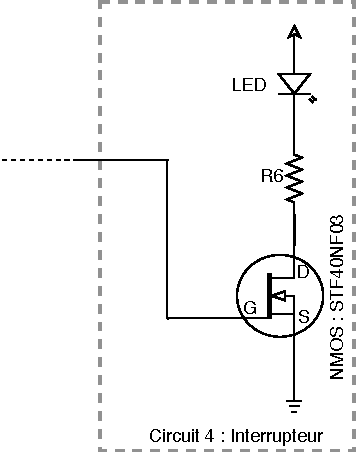
\includegraphics{HO3_MOS.pdf}
    \caption{Circuit de contrôle de la lampe}
    \label{fig:lampe}
\end{figure}

Apparu pour la première fois en 1963 dans les circuits électroniques, le \textbf{transitor} est à l'heure actuelle un des composants électroniques les plus utilisés. Sans le savoir, vous en avez déjà utilisés plusieurs: les différents circuits intégrés qui vous ont été fournis pendant les séances précédentes (i.e. le comparateur, le NE555 et le registre) sont eux-mêmes composés de transistors. \\

De manière intuitive, un transistor NMOS peut être vu comme un \textbf{interrupteur mécanique contrôlé en tension}. Lorsque le signal de contrôle (i.e. celui connecté au pôle G, pour \textit{gate} en anglais) est à une valeur haute, le transistor est en régime dit passant et laisse le courant passer entre la résistance (connectée au pôle D, pour \textit{drain} en anglais) et la masse (connectée au pôle S, pour \textit{source} en anglais). Dans ce cas-là, la LED est donc allumée. A l'opposé, lorsque le signal de contrôle est bas, le transistor est en régime coupé et ne laisse donc pas passer le courant. Dans ce cas-là, la LED est éteinte. Ajoutez maintenant le montage de la Figure \ref{fig:lampe} à votre système afin de finaliser le projet. \\

\begin{tcolorbox}

\textbf{ATTENTION:} Le système que nous vous avons proposé au cours des ces différents hands-on n'est \textbf{pas prévu} pour résister à n'importe quel type d'alimentation: brancher ce système à une prise d'alimentation générale 220V est \textbf{dangereux} (les composants ne sont pas conçus pour résister à de tels tensions/courants, ...) et peut s'avérer \textbf{mortel}! Si votre âme d'électronicien vous suggère de modifier le système afin de l'utiliser dans un autre projet, veuillez l'adapter en conséquence (nous pouvons vous aiguiller le cas échéant). Il est primordial de \textbf{rester vigilant} lorsque l'on manipule des circuits/systèmes électriques/électroniques.

\end{tcolorbox}
